\begin{frame}[parent={ie:agenda}, hasnext=false, hasprev=false]
	\frametitle{ISO 25000 - SQuaRE}

	\begin{block:concept}{SQuaRE}
		A série de normas 25000 ou SQuaRE (Systems and Software Quality Requirements
		and Evaluation) trata dos requisitos para planejamento e gerenciamento de
		requisitos associados aos requisitos e avaliação da qualidade de produtos
		de software.
	\end{block:concept}

	\begin{block:fact}{Quem ela substitui?}
		Aposenta a série de normas ISO/IEC 9126 e 14598.
	\end{block:fact}
	
	\begin{block:fact}{Com quem ela é compatível?}
		Processos técnicos relacionados a definição e análise de requisitos de
		qualidade das normas ISO/IEC 15288:2008 e 12207:2008.
	\end{block:fact}
		
	\note{
		\begin{itemize}
			\item ISO/IEC 15288:2008: Systems and software engineering -- System life cycle processes
			\item ISO/IEC 12207:2008: Systems and software engineering -- Software life cycle processes
		\end{itemize}
	}
\end{frame}


\begin{frame}[hasnext=true, hasprev=true]
	\frametitle{ISO 25000 - SQuaRE}

	\begin{block:fact}{Partes}
% % 		\begin{itemize}
% % 			\item ISO/IEC 2500n, Quality Management Division,
% % 			\item ISO/IEC 2501n, Quality Model Division,
% % 			\item ISO/IEC 2502n, Quality Measurement Division,
% % 			\item ISO/IEC 2503n, Quality Requirements Division,
% % 			\item ISO/IEC 2504n, Quality Evaluation Division.
% % 		\end{itemize}
		\centering
		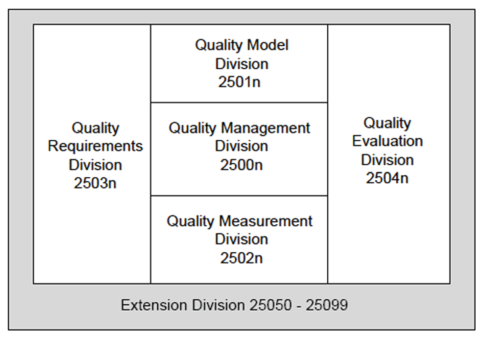
\includegraphics[width=.8\textwidth]{software-engineering/project-management/product/square}
	\end{block:fact}
\end{frame}



\begin{frame}
	\frametitle{ISO 2500n}

	\begin{block:concept}{ISO 2500n -- Gerenciamento de qualidade}
		\begin{itemize}
			\item Define modelos, termos e definições aplicáveis a todas as partes da série
			SQuaRE.
			
			\item Estabelece requisitos e diretivas para o planejamento e gestão
			associados aos requisitos e avaliação de qualidade de produto de software.
		\end{itemize}
	\end{block:concept}
	
	\begin{block:fact}{Documentos disponíveis}
		\begin{itemize}
			\item ISO/IEC 25000:2014 -- Guide to SQuaRE
		\end{itemize} 
	\end{block:fact}

	\note{
		Esta norma fornece requisitos e recomendações para uma organização responsável:
		\begin{itemize}
			\item por implementar e gerenciar a especificação de requisitos de qualidade
			do produto de software, e
			\item pelas atividades de avaliação de qualidade de software provento 
			tecnologia, ferramentas, experiências e habilidades de gestão.
		\end{itemize}
		
		Atividades:
		\begin{itemize}
			\item Motivar e treinar as pessoas para as atividades de especificação dos
			requisitos e para as atividades de avaliação,
			\item Preparar documentos apropriados,
			\item Identificar ou desenvolver métodos necessários e responder questões
			relacionadas às tecnologias que sejam relevantes.
		\end{itemize}

	}
\end{frame}

\begin{frame}
	\frametitle{ISO 2501n}

	\begin{block:concept}{ISO 2501n -- Modelo de qualidade}
		\begin{itemize}
			\item Define modelos de qualidade para produto de software, para qualidade
			em uso e dados.
		\end{itemize}
	\end{block:concept}

	\begin{block:fact}{Documentos disponíveis}
		\begin{itemize}
			\item ISO/IEC 25010:2011 -- System and software quality models
		\end{itemize} 
	\end{block:fact}

	\note{
	}
\end{frame}


\begin{frame}
	\frametitle{ISO 2502n}

	\begin{block:concept}{ISO 2502n -- Medição de qualidade}
		\begin{itemize}
			\item Define modelos de referência para medir a qualidade interna, externa
			e em uso do produto de software.
		\end{itemize}
	\end{block:concept}
	
	\begin{block:fact}{Documentos disponíveis}
		\begin{itemize}
			\item ISO/IEC 25020:2007 -- Measurement reference model and guide
			\item ISO/IEC 25021:2012 --Quality measure elements
			\item ISO/IEC 25022 -- Measurement of quality in use
			\item ISO/IEC 25023 -- Measurement of system and software product quality
			\item ISO/IEC 25024 -- Measurement of data quality
		\end{itemize} 
	\end{block:fact}

	\note{
		Equivalente à ISO 9126.
		
		Normas ISO/IEC 25022, 25023 e 25024 ainda não foram publicadas.
	}
\end{frame}


\begin{frame}
	\frametitle{ISO 2503n}

	\begin{block:concept}{ISO 2503n -- Requisitos de qualidade}
		\begin{itemize}
			\item Estabelece mecanismos para especificar requisitos de qualidade.
		\end{itemize}
	\end{block:concept}

	\begin{block:fact}{Documentos disponíveis}
		\begin{itemize}
			\item ISO/IEC 25030:2007 -- Quality requirements
		\end{itemize} 
	\end{block:fact}

	
	\note{
		ISO/IEC 2503n - Quality Requirements Division helps specifying quality
		requirements. These quality requirements can be used in the process of
		quality requirements elicitation for a product to be developed or as inputs
		for an evaluation process.
		
		The requirements definition process is mapped to Stakeholder Requirements
		Definition Process in Technical Processes defined in ISO/IEC 15288:2008 and
		ISO/IEC 12207:2008.
	}
\end{frame}


\begin{frame}
	\frametitle{ISO 2504n}

	\begin{block:concept}{ISO 2504n -- Avaliação de qualidade}
		\begin{itemize}
			\item Estabelece requisitos, recomendações e diretivas para a avaliação
			de produtos.
		\end{itemize}
	\end{block:concept}
	
	\begin{block:fact}{Documentos disponíveis}
		\begin{itemize}
			\item ISO/IEC 25040:2011 -- Evaluation process
			\item ISO/IEC 25041:2012 -- Evaluation guide for developers, acquirers and
			independent evaluators
			\item ISO/IEC 25045:2010 -- Evaluation module for recoverability
		\end{itemize} 
	\end{block:fact}
	
	
	\note{
		ISO/IEC 2504n - Quality Evaluation Division provides requirements,
		recommendations and guidelines for product evaluation, whether performed by
		independent evaluators, acquirers or developers. The support for documenting
		a measure as an Evaluation Module is also presented.
	
		Substitui a ISO/IEC 14598.
	}
\end{frame}
 

 \begin{frame}
	\frametitle{ISO 2505n}

	\begin{block:concept}{ISO 2505n -- Normas complementares}
		\begin{itemize}
			\item Normas complementares às anteriores.
			\item Normas para contextos específicos de aplicação.
		\end{itemize}
	\end{block:concept}
	
	\begin{block:fact}{Documentos disponíveis}
		\begin{itemize}
			\item ISO/IEC 25051 -- Requirements for quality of Ready to Use Software
			Product (RUSP) and instructions for testing
		\end{itemize} 
	\end{block:fact}
\end{frame}
 
 
\begin{frame}
	\frametitle{ISO 25010}
	\framesubtitle{Modelo de qualidade}

	\begin{block:fact}{Modelo de qualidade}
		\begin{itemize}
			\item Organizado em:
			\begin{itemize}
				\item Características internas e externas (características de produto)
				\item Características de software em uso
			\end{itemize}
			
			\item Todas as características possuem subcaracterísticas
		\end{itemize}
	\end{block:fact}
\end{frame}

\begin{frame}
	\frametitle{ISO 25010}
	\framesubtitle{Modelo de qualidade}
	
	\begin{block:fact}{Características de produto}
			\centering
			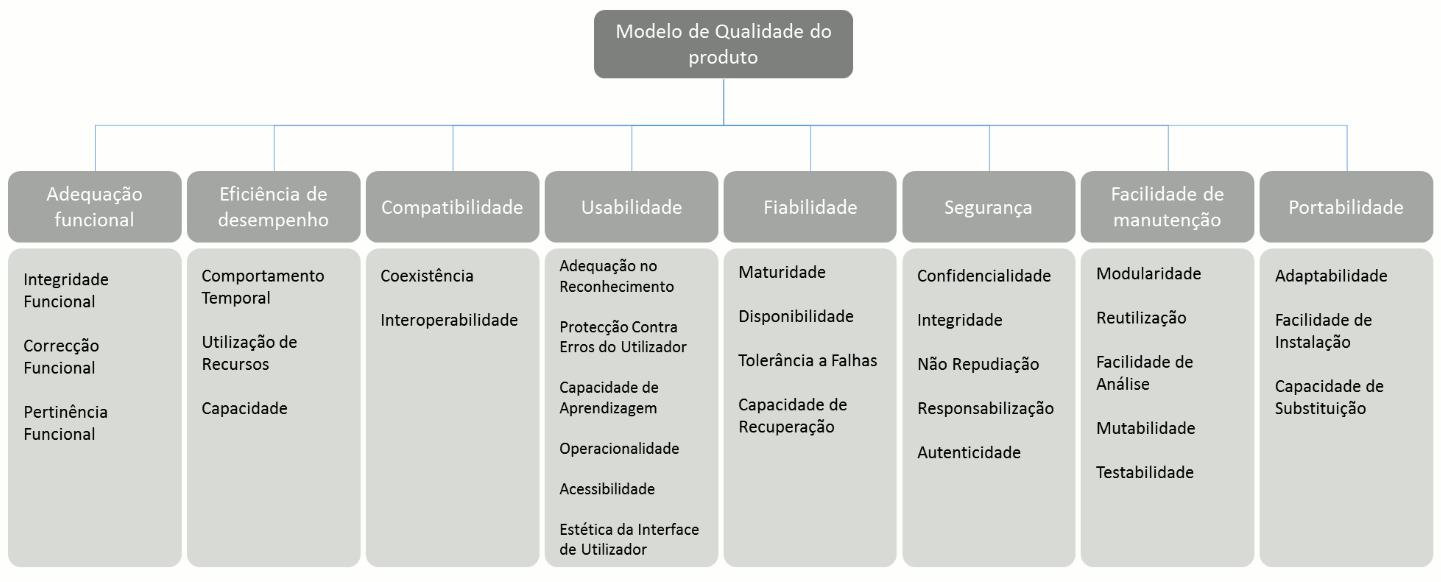
\includegraphics[width=\textwidth]{square-quality_model}
	\end{block:fact}
\end{frame}


 
\begin{frame}
	\frametitle{ISO 25010}
	\framesubtitle{Modelo de qualidade}

	\begin{block:fact}{Características de produto}
		\begin{itemize}
			\item Adequação funcional
			\item Confiabilidade
			\item Usabilidade
			\item Eficiência de desempenho
			\item \textbf{Segurança}
			\item Compatibilidade
			\item Capacidade de manutenção
			\item Portabilidade
		\end{itemize}
	\end{block:fact}
	
	\note{
		Principal mudança referente ao modelo anterior: segurança.
	
		Reflete uma necessidade e uma tendência em todos os setores da computação (vide IEEE/ACM CS 2013).	
	}
\end{frame}


\begin{frame}
	\frametitle{ISO 25010}
	\framesubtitle{Características de produto}

	\begin{block:fact}{Segurança}
		\begin{itemize}
			\item Confidencialidade
			\item Integridade
			\item Não repúdio
			\item Rastreabilidade de uso (\foreign{accountability})
			\item Autenticidade
		\end{itemize}
	\end{block:fact}
\end{frame}


 
\begin{frame}
	\frametitle{ISO 25010}
	\framesubtitle{Modelo de qualidade}

	\begin{block:fact}{Características de software em uso}
		\begin{itemize}
			\item Efetividade
			\item Eficiência
			\item Satisfação
			\item Uso sem riscos
			\item Cobertura de contexto
		\end{itemize}
	\end{block:fact}
\end{frame}

% 
%\begin{frame}
%	\frametitle{ISO 25010}
%	\framesubtitle{Características de software em uso}
%
%	\begin{block:fact}{Efetividade}
%		\begin{itemize}
%			\item Efetividade
%		\end{itemize}
%	\end{block:fact}
%\end{frame}
%
% 
%\begin{frame}
%	\frametitle{ISO 25010}
%	\framesubtitle{Características de uso}
%
%	\begin{block:fact}{Eficiência}
%		\begin{itemize}
%			\item Eficiência
%		\end{itemize}
%	\end{block:fact}
%\end{frame}
%
%
%\begin{frame}
%	\frametitle{ISO 25010}
%	\framesubtitle{Características de uso}
%
%	\begin{block:fact}{Satisfação}
%		\begin{itemize}
%			\item Utilidade
%			\item Prazer
%			\item Conforto
%			\item Confiança
%		\end{itemize}
%	\end{block:fact}
%\end{frame}
%
%\begin{frame}
%	\frametitle{ISO 25010}
%	\framesubtitle{Características de uso}
%
%	\begin{block:fact}{Uso sem riscos}
%		\begin{itemize}
%			\item Mitigação de risco econômico
%			\item Mitigação de risco a saúde e segurança
%			\item Mitigação de risco ambiental
%		\end{itemize}
%	\end{block:fact}
%\end{frame}
%
%
%\begin{frame}
%	\frametitle{ISO 25010}
%	\framesubtitle{Características de uso}
%
%	\begin{block:fact}{Cobertura de contexto}
%		\begin{itemize}
%			\item Completude de contexto
%			\item Flexibilidade
%		\end{itemize}
%	\end{block:fact}
%\end{frame}
